\chapter{ABNT} \label{chap:fundamentacao}

Este capítulo mostra como usar os macros específicos do pacote \abntex. Isso é apenas um resumo, consulte a documentação oficial.

\section{Alíneas}

Alíneas são listas, devemos usar o ambiente \texttt{alineas}, desta forma:

\begin{lstlisting}[float=htb, style=latexStyle, caption={Alíneas}, label=lst:alineas]
\begin{alineas}
	\item primeira alínea;                          % termina com ;
	\item segunda alínea                            % termina com :
	\begin{alineas}
		\item primeira subalínea da segunda alínea; % termina com ;
		\item última subalínea da segunda alínea.   % termina com .
	\end{alineas}
	\item última alínea.                            % termina com .
\end{alineas}
\end{lstlisting}

O texto que vem antes, geralmente, deve terminar com \enquote*{:}, desta forma: O \autoref{lst:alineas} vai gerar o seguinte:

\begin{alineas}
	\item primeira alínea;                          % termina com ;
	\item segunda alínea                            % termina com :
	\begin{alineas}
		\item primeira subalínea da segunda alínea; % termina com ;
		\item última subalínea da segunda alínea.   % termina com .
	\end{alineas}
	\item última alínea.                            % termina com .
\end{alineas}

\section{Citações}

O \template utiliza bibtex para gerenciar as referências do artigo, eles devem ser salvos no arquivo \bibfile, a sintaxe se assemelha ao que está descrito no \autoref{lst:bibtex-syntax}.

\begin{lstlisting}[float=htb, style=latexStyle, caption={Sintaxe bibtex}, label=lst:bibtex-syntax]
@book{knuth:aocp:1997,
	author = {Knuth, Donald E.},
	title = {The art of computer programming, volume 1 (3rd ed.): fundamental algorithms},
	year = {1997},
	isbn = {0201896834},
	publisher = {Addison Wesley Longman Publishing Co., Inc.},
	address = {USA}
}

@article{dijkstra:goto:1968,
	title={Go To Statement Considered Harmful},
	author={Dijkstra, Edsger W},
	journal={Communications of the ACM},
	volume={11},
	number={3},
	pages={147--148},
	year={1968},
	publisher={ACM New York, NY, USA}
}
\end{lstlisting}

\subsection{Citação indireta}

Para fazer uma citação indireta, é apenas necessário usar a macro \texttt{\textbackslash cite}, passando o id da referência. Como apresentando no \autoref{lst:indirect-citation}.

\begin{lstlisting}[float=htb, style=latexStyle, caption={Citação indireta}, label=lst:indirect-citation]
Programar pode ser bastante prazeroso \cite{knuth:aocp:1997}.
\end{lstlisting}

O resultado vai ser: Programar pode ser bastante prazeroso \cite{knuth:aocp:1997}.

Também pode-se usar a macro \texttt{\textbackslash citeonline} para adicionar o autor sem parênteses

\subsection{Citação direta}

Use o ambiente \texttt{citacao} como no \autoref{lst:direct-citation}.

\begin{lstlisting}[float=htb, style=latexStyle, caption={Citação direta}, label=lst:direct-citation]
\begin{citacao}
For a number of years I have been familiar with the observation that 
the quality of programmers is a decreasing function of the density of 
go to statements in the programs they produce. More recently I 
discovered why the use of the go to statement has such disastrous 
effects, and I became convinced that the go to statement should be 
abolished from all \enquote{higher level} programming languages. 
\cite{dijkstra:goto:1968}.
\end{citacao}
\end{lstlisting}

O resultado será:

\begin{citacao}
	For a number of years I have been familiar with the observation that 
	the quality of programmers is a decreasing function of the density of 
	go to statements in the programs they produce. More recently I 
	discovered why the use of the go to statement has such disastrous 
	effects, and I became convinced that the go to statement should be 
	abolished from all \enquote{higher level} programming languages. 
	\cite{dijkstra:goto:1968}.
\end{citacao}

Como o texto em questão está em inglês, deveríamos usar a opção \texttt{english}, desta forma: 
\texttt{\textbackslash begin\{citacao\}[english]}. O que vai deixar o texto em itálico:

\begin{citacao}[english]
	For a number of years I have been familiar with the observation that 
	the quality of programmers is a decreasing function of the density of 
	go to statements in the programs they produce. More recently I 
	discovered why the use of the go to statement has such disastrous 
	effects, and I became convinced that the go to statement should be 
	abolished from all \enquote{higher level} programming languages. 
	\cite{dijkstra:goto:1968}.
\end{citacao}

\section{Figuras}

Use o ambiente \texttt{figure} como no \autoref{lst:figure}, que produz a \autoref{fig:mqtt}.

\begin{lstlisting}[float=htb, style=latexStyle, caption={Adição de imagem}, label=lst:figure]
\begin{figure}[htb]
	\caption{Diagrama de sequência do processo de entrega de mensagens no \mqtt}
	\label{fig:mqtt}
	\centering
	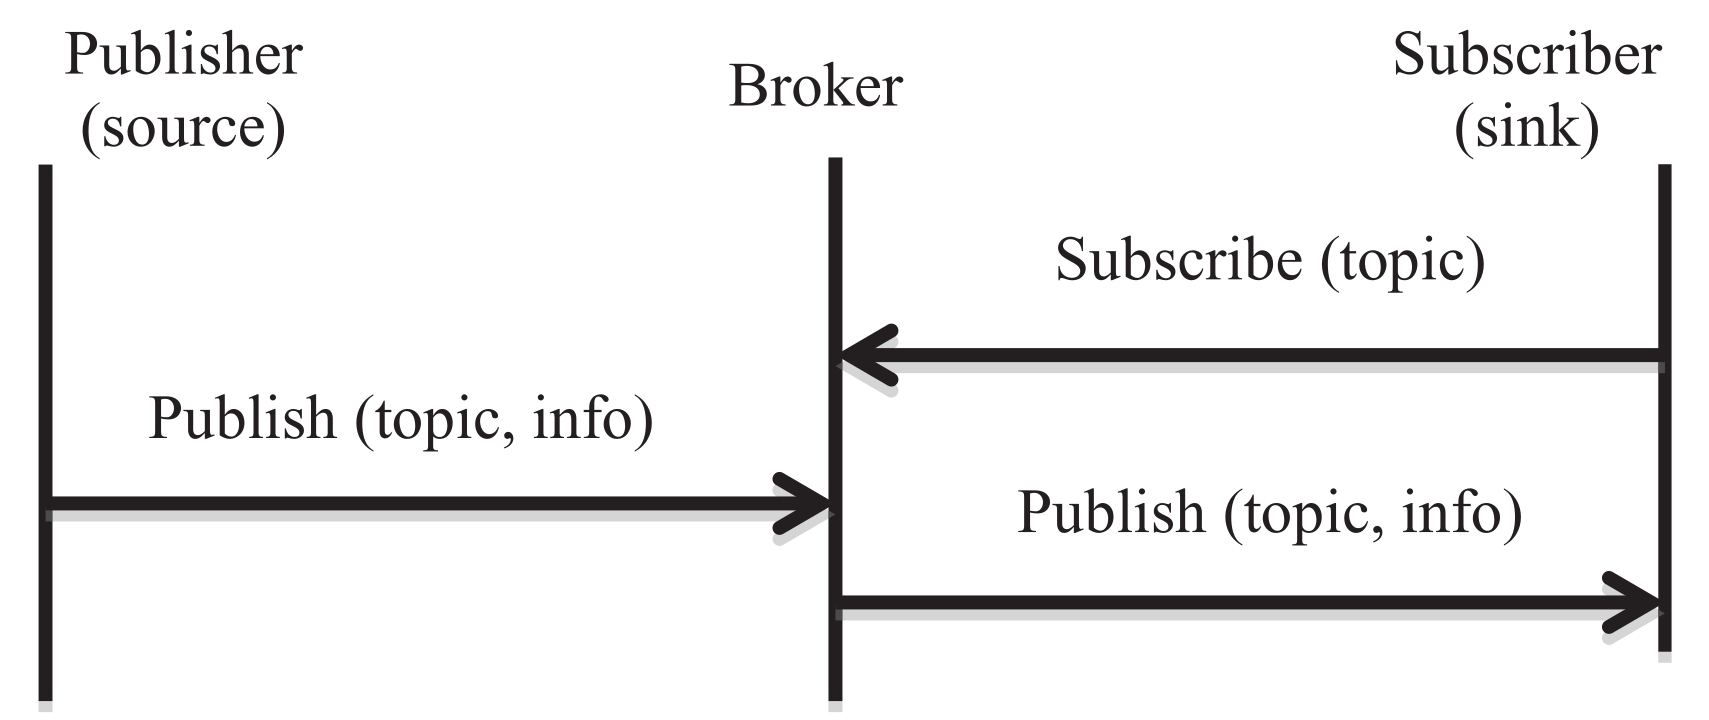
\includegraphics[width=0.85\linewidth]{\CurrentFilePath/res/img/mqtt-sequence.png}
	\fonte{\citeonline{al-fuqaha:et-al:2015}}
\end{figure}
\end{lstlisting}

\begin{figure}[htb]
	\caption{Diagrama de sequência do processo de entrega de mensagens no \mqtt}
	\label{fig:mqtt}
	\centering
	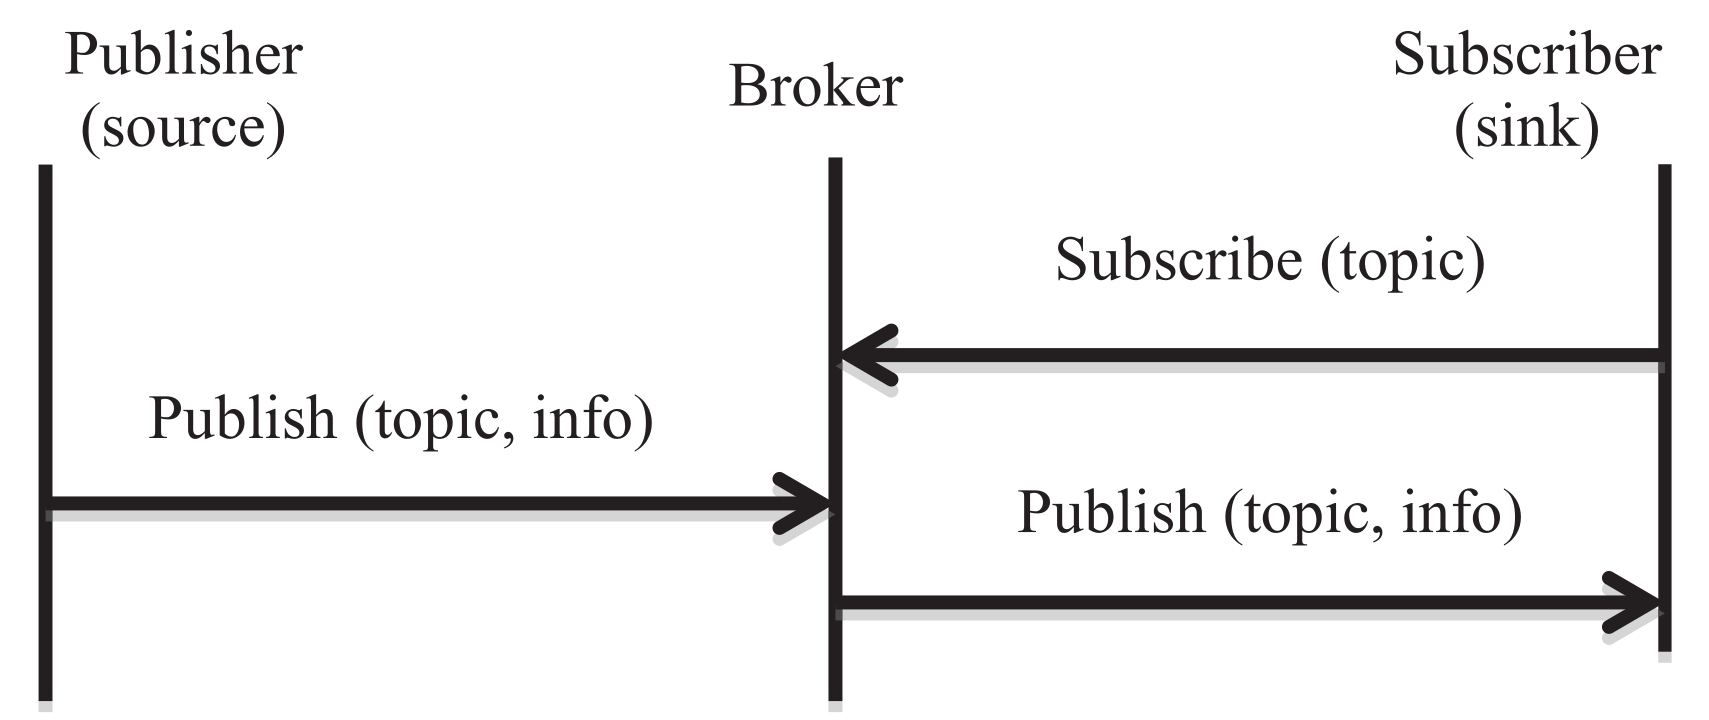
\includegraphics[width=0.85\linewidth]{\CurrentFilePath/res/img/mqtt-sequence.png}
	\fonte{\citeonline{al-fuqaha:et-al:2015}}
\end{figure}

\section{Tabelas}

Tabelas no padrão ABNT têm uma sintaxe complicada, copie e cole o \autoref{lst:tab} altere os dados, ele vai gerar a \autoref{tab:fake}.

\begin{lstlisting}[float=htb, style=latexStyle, caption={Tabela}, label=lst:tab]
\begin{table}[htb]
	\begin{center}
		\IBGEtab{
			\caption{Exemplo}
			\label{tab:fake}
		}{
			\begin{tabular}{lcr} % left, center, right
				\toprule
				\textbf{Col 1} & \textbf{Col 2} & \textbf{Col 3} \\
				\midrule
				Texto          & Outro texto    & Mais texto \\
				1.1            & $\log_2 n $    & 3.14 \\
				\bottomrule
			\end{tabular}
		}{
			\fonte{\autoriapropria}
		}
	\end{center}
\end{table}
\end{lstlisting}

\begin{table}[htb]
	\begin{center}
		\IBGEtab{
			\caption{Exemplo}
			\label{tab:fake}
		}{
			\begin{tabular}{lcr} % left, center, right
				\toprule
				\textbf{Col 1} & \textbf{Col 2} & \textbf{Col 3} \\
				\midrule
				Texto          & Outro texto    & Mais texto \\
				1.1            & $\log_2 n $    & 3.14 \\
				\bottomrule
			\end{tabular}
		}{
			\fonte{\autoriapropria}
		}
	\end{center}
\end{table}

Você vai encontrar outras tabelas nesse capítulo, consulte o código fonte desse documento caso queira ver como são construídas.

\begin{table}[htb]
	\begin{center}
		\IBGEtab{
			\caption{Dados de leitura por país}
			\label{tab:books}
		}{
			\begin{tabular}{lcc}
				\toprule
				\textbf{País}  & \textbf{Livros lidos por ano (média)} & \textbf{Gênero mais popular} \\
				\midrule
				Brasil         & 4,7                                   & Ficção \\
				Estados Unidos & 10                                    & Ficção \\
				Japão          & 12                                    & Mangás \\
				Alemanha       & 12                                    & Ficção \\
				França         & 21                                    & Romances \\
				Índia          & 4,7                                   & Ficção \\
				\bottomrule
			\end{tabular}
		}{
			\fonte{ChatGPT :)}
		}
	\end{center}
\end{table}

\begin{table}[htb]
	\begin{center}
		\IBGEtab{
			\caption{Performance}
			\label{tab:exp-perf}
		}{
			\begin{tabular}{lccccc}
				\toprule
				                & Média & Desvio padrão & Mínimo & Máximo & Intervalo de 95\% de confiança \\
				\midrule
				$\Delta t$ (ms) & 20.1  & 3.7           & 7.0    & 78.9   & 20.1 $\pm$ 0.03 \\
				\bottomrule
			\end{tabular}
		}{
			\fonte{\autoriapropria}
		}
	\end{center}
\end{table}

\section{Estrangeirismos}

Utilize o comando \texttt{\textbackslash foreign} para deixar o termo em itálico. Tome como exemplo o \autoref{lst:loanword}, ele gerará o seguinte paragrafo, com a palavra \enquote{\dataset} em itálico:

Para a análise estatística, foi necessário utilizar um 
\foreign{dataset} abrangente, contendo uma grande quantidade 
de dados que permitiram gerar insights significativos 
sobre o comportamento do usuário.

\begin{lstlisting}[float=htb, style=latexStyle, caption={Estrangeirismos}, label=lst:loanword]
Para a análise estatística, foi necessário utilizar um 
\foreign{dataset} abrangente, contendo uma grande quantidade 
de dados que permitiram gerar insights significativos 
sobre o comportamento do usuário.
\end{lstlisting}

Não existe uma regra, mas entende-se que algumas palavras já sofreram aportuguesamento e não necessitam de grafia especial, o \href{https://www12.senado.leg.br/manualdecomunicacao/verbetes-acessorio/estrangeirismos-grafados-sem-italico-ou-aspas}{manual da SECOM} pode ser usado como referência.

